% ===================================================================================== %
%                                        Header                                         %
% ===================================================================================== %
\documentclass[12pt]{WisconsinThesis}

%\usepackage{lipsum}
%\usepackage{bookmark}
%\usepackage{import}
%\usepackage{mathtools}
\usepackage{float}
\usepackage[noabbrev]{cleveref}
\usepackage[font=it]{caption}
\creflabelformat{equation}{#2#1#3}

\newcommand{\Helm} {\ensuremath{\phi        (\rho,T)}\xspace}
\newcommand{\HelmO}{\ensuremath{\phi\sups{o}(\rho,T)}\xspace}
\newcommand{\HelmR}{\ensuremath{\phi\sups{r}(\rho,T)}\xspace}
\newcommand{\Psat}{\ensuremath{P\subs[\!\!]{sat}}\xspace}
\newcommand{\Tsat}{\ensuremath{T\subs[\!\!\:]{sat}}\xspace}
\newcommand{\rhol}{\ensuremath{\rho\subs[\!\!\:]{\rule{0pt}{8pt}$\textstyle\ell$}}\xspace}
\newcommand{\rhog}{\ensuremath{\rho\subs[\!\!\:]{$\mathit{g}$}}\xspace}
\newcommand{\Skip}[1][0.45em]{\\[#1]}
\newcommand{\TCS}    {Thermodynamic Coexistence System\xspace}
\newcommand{\TCSRef} {\hyperref[Eqn:TCS]{\TCS}\xspace}
\newcommand{\MCS}    {Mechanical Coexistence System\xspace}
\newcommand{\MCSRef} {\hyperref[Eqn:MCS]{\MCS}\xspace}

\newcommand{\HFE}{Helmholtz free energy\xspace}

\begin{document}
\setcounter{chapter}{1}
\pagenumbering{arabic}

\section{Governing Equations}
For a one-dimensional, single phase, non-reacting flow, there are three mechanical balance equations that are closed by a thermodynamic equation of state and constitutive equations.
The three balance equations are those of mass, momentum, and energy:
\begin{subequations}\label{Eqn:BalanceLaws}
    \begin{align}
        \pdiff{\rho   }{t} + \pdiff{\rho{u}}{x}          &= 0                           \label{Eqn:CoM} \Skip
        \pdiff{\rho{u}}{t} + \pdiff{[u\,\rho{u} + P]}{x} &= \pdiff{\tau}{x} + \rho{g}   \label{Eqn:CoP} \Skip
        \pdiff{\rho{i}}{t} + \pdiff{(u[\rho{i} + P])}{x} &= Q\subs{add},                \label{Eqn:CoE}
    \end{align}
\end{subequations}
where $\rho$ is density, $u$ is the velocity, $P$ is the pressure, $\tau$ is the shear stress, $g$ is a gravitational constant, $i$ is internal energy, and $Q\subs{add}$ is an external source of heat.
It should be noted that \cref{Eqn:CoE} is actually the balance of thermal energy and is only valid for low velocity flows such that kinetic energy may be neglected.

The unknowns in the balance equations are the density, velocity, internal energy, pressure, shear stress, and heat source; the system is underdetermined.
To close the system, it is assumed that the fluid is in thermal equilibrium (in addition to mechanical) and that, if unspecified, constitutive relations exist such that the shear stress and heat source are a functions of the fluid's state.
Assuming the fluid is in thermal equilibrium permits the use of a thermodynamic equation of state to calculate pressure and any other required properties for the constitutive relations.
Thus, the system is closed and can be solved given adequate boundary and initial conditions.

The equation of state to be considered, and used, is the IAPWS-95 formulation.  This formulation uses a high-accuracy curve fit of the \HFE function $f$ whose natural variables are density and temperature.  
Since it will mentioned later, the non-dimensional \HFE function $\phi$ is the form primarily used in the IAPWS-95 relations and is related to $f$ by
\begin{equation}
    \frac{f(\rho,T)}{R\,T} = \Helm = \HelmO + \HelmR, \notag
\end{equation}
where the superscript ``o'' denotes the ideal gas behavior and ``r'' denotes the residual (i.e., non-ideal gas) behavior of the potential.

\section{Calculation of Liquid-Gas Equilibrium}
One of the important parts of modeling water flows with a real equation of state is the determination of phase change.
A significant portion of water's $T$-$\rho$ space that is commonly used in industrial applications has a region where both its liquid and gas phases can coexist.
During a simulation, determination of whether the water's state is one of coexistence is key.
Outlined below are two systems that can be used to determine a two-phase state.


\subsection{Thermodynamic Coexistence System}
Calculation of saturated properties from the IAPWS-95 equation of state involves leveraging the three equilibrium conditions of phase change: constant pressure, constant temperature, and phasic equality of Gibbs free energy.  
In terms of the non-dimensional \HFE function \Helm, these equilibrium conditions form a system of equations that must be simultaneously satisfied:
\begin{subequations}\label{Eqn:TCS}
    \begin{align}
        \frac{\Psat}{R\,\Tsat} &= \rhol \left[1 + \rhol \pdiff{\phi\sups{r}}{\rho}(\rhol,\Tsat) \right] \label{Eqn:TCS:Pmatch1}\Skip
        \frac{\Psat}{R\,\Tsat} &= \rhog \left[1 + \rhog \pdiff{\phi\sups{r}}{\rho}(\rhog,\Tsat) \right] \label{Eqn:TCS:Pmatch2}\Skip
        \frac{\Psat}{R\,\Tsat} \left[\oneo{\rhog} - \oneo{\rhol}\right] &= \ln\!\left(\frac{\rhol}{\rhog}\right) +
        \phi\sups{r}(\rhol,\Tsat) - \phi\sups{r}(\rhog,\Tsat) \label{Eqn:TCS:MaxwellCriterion}.
    \end{align}
\end{subequations}
\Cref{Eqn:TCS:Pmatch1,Eqn:TCS:Pmatch2} arise from the definition of pressure in terms of the \HFE and the pressure equality of the functions given the saturated liquid density \rhol and gas density \rhog at the saturation temperature.
\Cref{Eqn:TCS:MaxwellCriterion} is the Maxwell construction (i.e., equal area rule) of the Gibbs free energy equivalence.  
The above system consists of three equations and four unknowns: \Psat, \Tsat, \rhol, and \rhog; therefore, the system can be solved once one of the saturation values is specified.

This system will be referred to as the Thermodynamic Coexistence System (TCS) since the solution relies upon the classic thermodynamic state variables pressure, temperature, and volume (inverse density).  
This definition is made to distinguish it from the time evolution friendly system outlined below.


\subsection{Mechanical Coexistence System}
Temperature is a very powerful state variable because it is a directly measurable quantity that provides a qualitative measurement of a fluid's internal energy.
However, in the balance equations (\ref{Eqn:BalanceLaws}), density and internal energy are the variables that are mechanically balanced independent of thermodynamics.
As such, it is most natural to update the thermodynamic and transport quantities with the mechanically specified density and internal energy to have a consistent evolution system.
Furthermore, since density and internal energy are defined and independent in the two-phase region (unlike pressure and temperature), the time evolution may lead to so-called mixture quantities that are linear combinations of the saturated quantities.
Mixture quantities are traditionally defined by a mass ratio of gas to total called the quality, $x$, which is a new unknown.
Accounting for all of the above notes, the so-called Mechanical Coexistence System is defined by:
\begin{subequations}\label{Eqn:MCS}
    \begin{align}
        \frac{\Psat}{R\,\Tsat} &= \rhol \left[1 + \rhol \pdiff{\phi\sups{r}}{\rho}(\rhol,\Tsat) \right]     \label{Eqn:MCS:Pmatch1}             \Skip
        \frac{\Psat}{R\,\Tsat} &= \rhog \left[1 + \rhog \pdiff{\phi\sups{r}}{\rho}(\rhog,\Tsat) \right]     \label{Eqn:MCS:Pmatch2}             \Skip
        \frac{\Psat}{R\,\Tsat} \left[\oneo{\rhog} - \oneo{\rhol}\right] &= 
        \ln\!\left(\frac{\rhol}{\rhog}\right) + \phi\sups{r}(\rhol,\Tsat) - \phi\sups{r}(\rhog,\Tsat)       \label{Eqn:MCS:MaxwellCriterion}    \Skip
        i\subs{mix} &= [1 - x]\,i(\rhol,\Tsat) + x\,i(\rhog,\Tsat)                                          \label{Eqn:MCS:LeverRule}           \Skip
        \oneo{\rho\subs{mix}} &= \frac{1 -x}{\rhol} + \frac{x}{\rhog}.                                      \label{Eqn:MCS:Quality}             
    \end{align}
\end{subequations}
\Cref{Eqn:MCS:Pmatch1,Eqn:MCS:Pmatch2,Eqn:MCS:MaxwellCriterion} are identical to those in \cref{Eqn:TCS} since the change in the supplied variables doesn't remove the fundamental requirements of phase equilibrium.
Instead, the usage of mixture density and internal energy requires that the system have knowledge of the lever rule as defined by \cref{Eqn:MCS:LeverRule,Eqn:MCS:Quality} such that a unique state can be found.
Unlike \cref{Eqn:TCS} where any of the four unknowns could be specified for solution, \cref{Eqn:MCS} takes the mixture density and internal energy to solve for the five unknowns: \Psat, \Tsat, \rhol, \rhog, and $x$.
The function $i(\rho,T)$ returns the internal energy as defined by relations to the \HFE function and is precluded for brevity.

\subsection{Two-Phase Determination}
While \cref{Eqn:TCS,Eqn:MCS} present systems that need to be solved, they do not outline an algorithm to determine if a state is two-phase.
Two quantities are needed to define a unique state.  
Since the \HFE function's natural variables are density and temperature, it seems appropriate to use them for two-phase determination.

\begin{figure}[h!]%
    %\begin{center}
    \centering{
        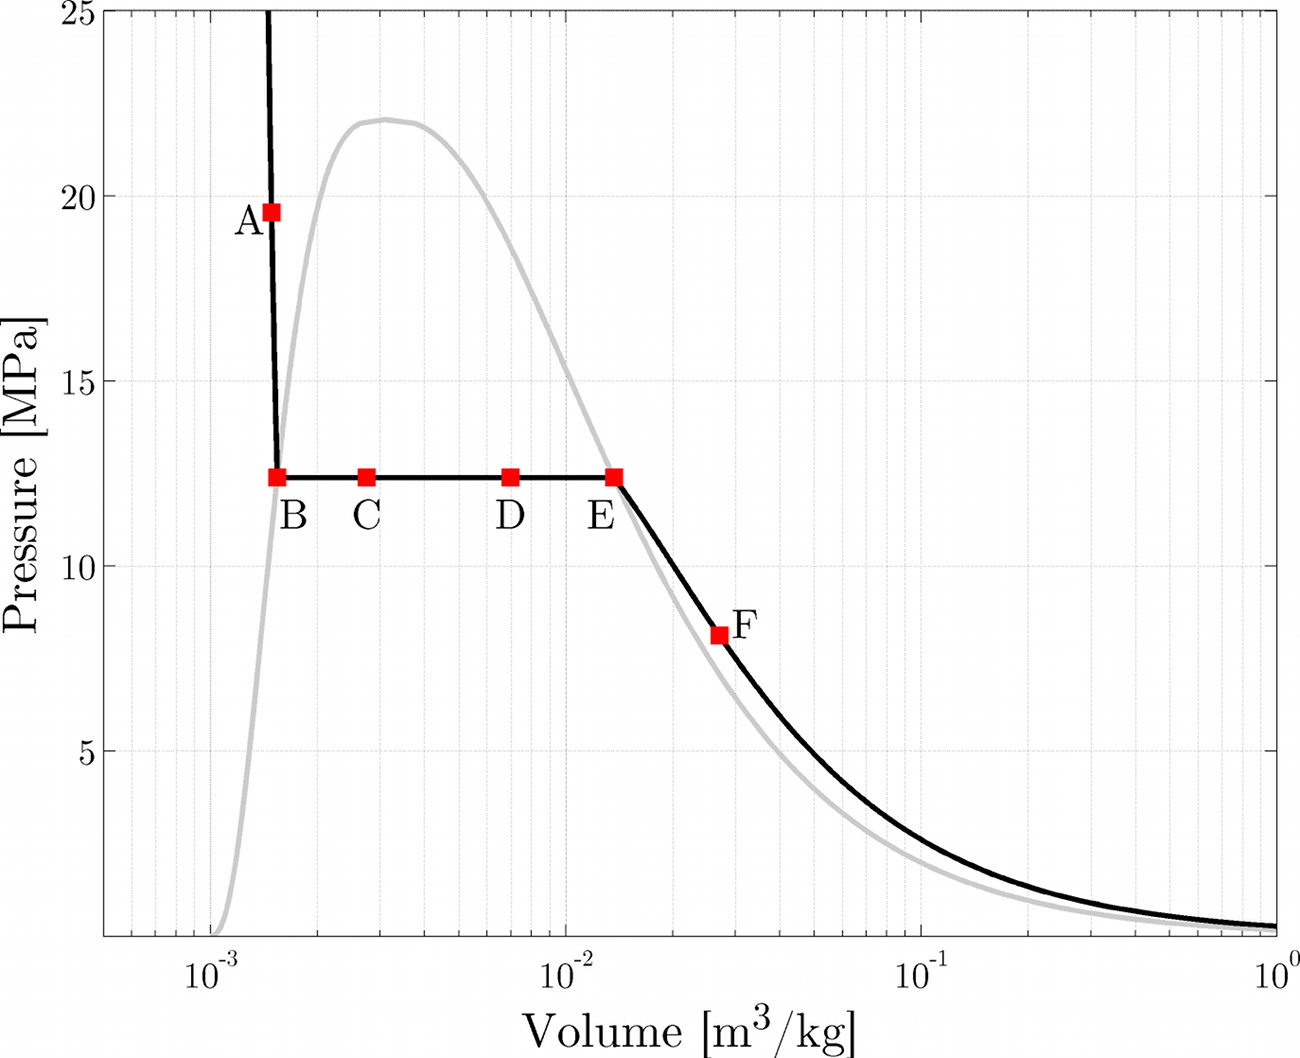
\includegraphics[scale=0.65]{Plot_Small}%
        \caption{P-v plot using the IAPWS-95 formulation with the vapor dome (grey line) and a 600 K isotherm (black).}%
        \label{Fig:IsothermPlot}}
    %\end{center}
\end{figure}

For example, there is a single control volume in a simulation that has a temperature $T\subs{sim}$ and density $\rho\subs{sim}$.
Therefore, ignoring $\rho\subs{sim}$, the state of this control volume can lie anywhere along the isotherm in \cref{Fig:IsothermPlot}.
Using $T\subs{sim}$ along with \cref{Eqn:TCS}, the saturated volumes at points B and E can be calculated by satisfying the coexistence system.
If the control volume's density lies between these saturated points (e.g., C or D), then the control volume is two-phase.
It is just as valid to use the control volume's density $\rho\subs{sim}$ to find \Tsat and if $T\subs{sim}$ is below Tsat, the control is two-phase.

While the above example works perfectly for the \TCS, the \MCS, which uses internal energy in place of temperature, is less flexible.
If \cref{Eqn:MCS} were solved for any density and internal energy, the solution may fail to converge or produce spurious results.
This problem stems from having an unknown quality $x$ that could take on values outside of its defined range (0 to 1, inclusive) during solution for a single-phase mixture.
As such, a stable algorithm for solving the \MCSRef given a density $\rho\subs{sim}$ and internal energy $i\subs{sim}$ is
\begin{enumerate}
    \item{Using $\rho\subs{sim}$, solve \cref{Eqn:TCS} for \Tsat.}
    \item{Calculate $i\subs{sat}$ using $\rho\subs{sim}$ and \Tsat.}
    \item{There are now three determinations:
    \begin{enumerate}
        \item{If $i\subs{sim}$ is less    then $i\subs{sat}$ and $\rho\subs{sim}$ is less    than $\rho\subs{c}$, the system is two-phase.}
        \item{If $i\subs{sim}$ is greater then $i\subs{sat}$ and $\rho\subs{sim}$ is greater than $\rho\subs{c}$, the system is two-phase.}
        \item{Otherwise, the system is single phase.}
    \end{enumerate}
    }
    \item{If the mixture is two-phase, solve \cref{Eqn:MCS} using $\rho\subs{sim}$ and $i\subs{sim}$ .}
\end{enumerate}
The comparisons in step number 3 is similar to saturation temperature-density comparison made for the \TCS but is complicated by internal energy not being constant in the vapor dome.
Step 4 is only required if the exact state of the substance is required (e.g., quality and temperature are needed in a calculation).

\end{document}

